\subsection{The results match} 
Running the Gezel with the two approaches described above yields the results shown in figure \ref{fig:Cd1d2}. As seen in the figure, the results in C and the results from the hardware implementations (approach 1 and approach 2) 
match perfectly, i.e. the 250 sets of filtered data points differ by 0. (investigated in \texttt{MATLAB})

\begin{figure}[H]
    \centering
    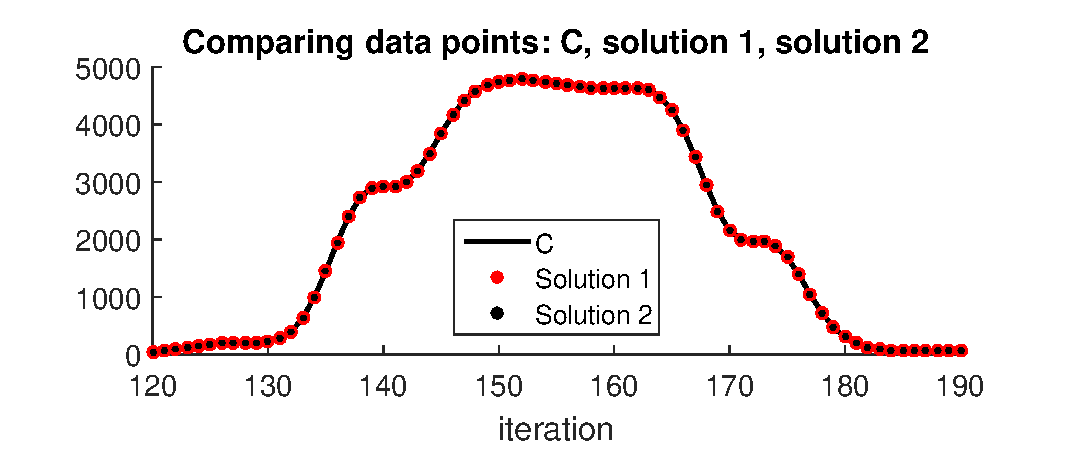
\includegraphics[width=1.0\textwidth]{3Results/fig/Cd1d2.eps}
    \caption{Comparing the data points found in C, in Gezel using approach 1 (Co-P on bus), and approach 2 (Co-P linked to CPU). The three sets of filtered data are exact matches for all 250 data points.}
    \label{fig:Cd1d2}
\end{figure}

In A2 we found that the filtered values obtained using the customized processor matched perfectly with values from C, so we can safely conclude that the following 4 implementations produce the same result when applying the MWI filter:

\begin{itemize}
    \item The filtering program in C (A1)
    \item The customized processor in Gezel (A2)
    \item The Co-P communicating through the bus in Gezel (A3)
    \item The Co-P linked directly to the CPU in Gezel (A3)
\end{itemize}

Now that we have established that all 4 implementations yield the same results, the important question is: which one has the best performance? While it is difficult to compare software and hardware solution (as we discussed in A2, section 4.2), we can compare the 3 hardware implementations: the two Co-P implementation of assignment 3, and the customized processor implemented in assignment 2.

\subsection{Performance: speed}\label{sec:performanceSpeed}

\textbf{Cycles:} The two Co-P implementations require a different amount of cycles to apply the filter to all 250 data points: \\

Approach 1 needs 7780 cycles, and approach 2 needs 5260 cycles. This means that both designs use fewer cycles than the design from assignment 2 which used 11030 cycles. \\

\textbf{Critical path:} In assignment 2, the most critical path was evaluated and a very rough estimate of the clock period was performed.\footnote{If one wishes to see such an estimate, see our report from assignment 2, section 4.2.} This assignment we focus on comparing the different hardware implementations and therefore we compare cycles directly. We do not try and calculate the clock period, as it could be a misleading representation of performance. 

\subsection{Performance: energy use}\label{sec:performanceEnergy}

For the first design, the amount of activity is seen in figure \ref{fig:ToggleCount1}. The design performs 91k register toggles and 108k signal toggles. 

\begin{figure}[H]
    \centering
    \includegraphics[width=0.7\textwidth]{3Results/fig/Sequential_W_BUS}
    \caption{Toggle count from Gezel analysis for design 1.}
    \label{fig:ToggleCount1}
\end{figure}

For the second design, the amount of activity is seen in figure \ref{fig:ToggleCount2}. The design performs 74k register toggles and 85k signal toggles.

\begin{figure}[H]
    \centering
    \includegraphics[width=0.7\textwidth]{3Results/fig/Parallel_WO_BUS}
    \caption{Toggle count from Gezel analysis for design 2.}
    \label{fig:ToggleCount2}
\end{figure}

Compared to the design from assignment 2 which performed 102k register toggles and 168k signal toggles\footnote{See our report from assignment 2, performance section, for further information.}, the chosen approaches are superior regards to energy usage.

\subsection{Performance discussion}\label{sec:performanceDiscussion}

The comparisons between the implementations is seen in table \ref{tab:performance}, and table of normalized comparison is  seen in table \ref{tab:performanceNorm}.


\begin{table}[H]
    \centering
    \begin{tabular}{|c|c|c|c|c|}
    \hline 
    \textbf{Solution}   & \textbf{Cycles} & \textbf{Cycles pr data point} & \textbf{Register toggles} & \textbf{Signal toggles} \\ \hline
    Solution 1 & 7780   & 31.12 $\approx$ 31           & 91165            & 108515         \\ \hline
    Solution 2 & 5260   & 21.04 $\approx$ 21           & 74184            & 85747          \\ \hline
    A2       & 11030  & 44.12 $\approx$ 44           & 102639           & 168231         \\ \hline
    \end{tabular} 
    \caption{Comparing performance for the 3 hardware solutions.}
    \label{tab:performance}
\end{table}

\begin{table}[H]
    \centering
    \begin{tabular}{|c|c|c|c|c|}
    \hline 
    \textbf{Solution}   & \textbf{Cycles} & \textbf{Cycles pr data point} & \textbf{Register toggles} & \textbf{Signal toggles} \\ 
     & (norm.) & (norm.) & (norm.) & (norm.) \\\hline
    Solution 1 & 0.71   & 0.71          & 0.89            & 0.65         \\ \hline
    Solution 2 & 0.48   & 0.48           & 0.72            & 0.51          \\ \hline
    A2       & 1.00  & 1.00           & 1.00           & 1.00         \\ \hline
    \end{tabular} 
    \caption{Comparing performance for the 3 hardware solutions, normalized with respect to A2 values.}
    \label{tab:performanceNorm}
\end{table}

Solution 2 is the clear winner; while the number of register toggles was only reduced by 28\%, the number of cycles is reduced 52\%, roughly equivalent to a speedup factor of 2. \\

\textbf{Potentially shorter clock cycle:} As it clearly shows from table \ref{tab:performanceNorm}, solution 2 uses fewer cycles and has fewer activities. As previously mentioned in the Design section, the two processors may have different clock periods using design 2. The CPU controls the BUS which has a most critical path of a few register and signal toggles. The clock period for the CPU can therefore be shortened, compared to the Co-P. An alternative could be to elongate the Co-P clock period, reducing energy usage. Since both processors needs a handshake to swap data, no data is lost if the CPU is no longer the bottleneck. \\

From assignment 2, we saw that saving data to memory using the BUS result in 2270 cycles, therefore loading the new data point and then saving uses $2270 \cdot 2 = 4540$ cycles. This means that the Co-P indeed calculates while the BUS is active. The remaining $5260-4540 = 720$ clock cycles, corresponding to $740/250 = 2.88 \approx 3$ cycles per data point is mainly for the handshake between CPU and Co-P. \\

Concluding that solution 2 not only uses fewer cycles and toggles, but also has a potentially shorter clock cycle. 

\subsection{Extra}

\textbf{Early optimization:} In A2, we customized the processor to improve performance. As described in section \ref{sec:structuralOrBehavioralDesign} and \ref{sec:structuralOrBehavioralImplementation}, both the CPU and co-processors in our A3 solutions are based on the A2 processor, so they deviate from the template. We examined the consequences from changing the template; the change did not cause any loss of information.\footnote{For details, see A2 section 3.4.} \\

\textbf{Co-processor on the BUS:} As described throughout the report, solution 1 follows the suggested approach: connecting the co-processor and the CPU through the BUS. Solution 2, which has shown to be superior in all aspects, deviates from the given template, since it utilizes a direct link between the CPU co-processor. This enables them to perform actions in parallel without being limited by the BUS. 

%Hvis jeres resultater har givet anledning til helt nye løsninger, som ikke benytter de udleverede Gezel templates, og hvor I har lavet en ny (eller udvidet) løsning på opgaven, så beskriv kort de væsentligste design og implementeringer (herunder et diagram), samt hvad det betyder for perfomance.